\documentclass[11pt]{article}

\usepackage{setspace}
\usepackage[letterpaper,margin=1in]{geometry}
\usepackage[parfill]{parskip}
\usepackage{tikz}

\title{CS Capstone: RSA - Cryptosystem Tool \& Cognitive Analysis }
\author{George Wood}
\date{May 2018}

\begin{document}
\maketitle

\thispagestyle{empty}

\section{My Capstone Experience}
The process of the completion of my capstone, an RSA cryptosystem tool implemented in C++, has been long, confusing, and complicated. However, after all of the time and effort that has been poured into it, I can easily say that it has been the most fulfilling and high-quality software project that I have ever produced, independently or otherwise. In order to complete it, it was necessary to make use of my knowledge of object-oriented programming, filesystems, external libraries, and computer security, among many other aspects of my education at Truman.

Development of this project has spanned since roughly October of 2017, and has been quite time-intensive. Many setbacks and modifications were experienced with the specifics of the implementation, changes were made to the desired result of the project, and at one time there was the potential for it to be utilized in a research project. Despite the tumultuous nature of its development, I feel that the end result of these various changes is a notable personal accomplishment in programming, project management, and cybersecurity.

In addition to this paper serving as the writeup for my computer science capstone, to fulfill the final requirement of my cognitive science minor, a cognitive-science based analysis of RSA and why it could not feasibly be used prior to modern computers is provided in section 1.2 below. 

\subsection{Project Description}
The program that I have produced is a fully-functioning RSA cryptosystem tool. RSA -- short for Rivest-Shamir-Adleman, the last names of the scientists behind its creation -- is a cryptosystem primarily used for secret sharing. It operates under the concept of public-key cryptography. Public-key cryptography makes use of both a public key and a private key, where messages encrypted with the public key can only be decrypted with the private key, and vice versa. In the specific context of RSA, the following values are utilized for the keys:

\begin{itemize}
\item
{
The prime numbers used to determine the value of the modulus value (described below), generally notated as $p$ and $q$. These values are often extremely large, making the process of ensuring that they are prime a notable challenge. Although RSA technically still functions if $p$ and $q$ are not prime, the renowned security of RSA relies of the difficulty of the factorization problem, which is weakened substantially if these values are not prime. These two values cannot be equal to each other, but should generally be similar in size, differing by no more than a few bits.
}
\item
{
The modulus value used in internal calculations, generally notated as $n$. The size of $n$ in bits corresponds to the size of the private key $d$ in bits. RSA, unless non-conventionally implemented as a block cipher, cannot encrypt data that is larger than the size of $n$ in bits. $n$ can be of smaller bitlength than is specified by the type of RSA without damaging the functionality of the system, but the implementation used in this software guarantees that $n$ will be exactly the specified size, such as 2048 bits. An additional value related to $n$, $\phi(n)$, is essential to calculating the value of the private key. Both $n$ and $\phi(n)$ are generated with the values $p$ and $q$, as shown below:
\begin{center}
$n = p * q$

$\phi(n) = (p - 1)(q - 1)$
\end{center}
}

\item
{
The public key, generally notated as $e$. This key does not need to be kept confidential, and can often just be a small number, such as $3$. $e$ should be smaller than and must be relatively prime with $\phi(n)$, so while it does not need to be a prime number, having it be prime guarantees that it will be relatively prime with any number. It can, generally speaking, just be selected randomly, as a large value for $e$ will result in a slower data processing speed, but is not necessarily stronger, as the key will be public in the first place.
}
\item
{
The private key, generally notated as $d$. The secrecy of this key is crucial for maintaining the confidentiality and privacy of any and all information processed by RSA. It is generally an extremely large number, very similar to the size of $n$. Under this implementation, similarly to $n$, it is guaranteed to be the size specified by the type of RSA being used. While this is not necessary for RSA to function, it is part of the FIPS guidelines. The value of $d$ is calculated using the modular multiplicative inverse of $e$ and $\phi(n)$, as shown below:
\begin{center}
$d = e^{-1} mod$ $\phi(n)$

\end{center}
}

\end{itemize}

The capabilities and features of my implementation are as follows:
\begin{itemize}
\item
{FIPS Compliance (with one exception)
	\begin{itemize}
	\item
	{Every aspect, with one exception, of the program follows the specifications set by NIST (National Institute of Standards and Technology) in their FIPS (Federal Information Processing Standards) publications. These collections of standards set the requirements and guidelines of software that is to be used in a federal or otherwise security-critical context. They provide formal -- albeit sometimes unclear -- statements and descriptions of implementation features that have been determined to provide the degree of security and confidence that would be required in high-security contexts.
		\begin{itemize}
		\item
		{The only aspect of the entirety of my code that is not compliant with FIPS standards lies within the random number generator that I created (discussed in further detail later). True FIPS-compliance in random number generation requires an external noise source, such as the famously reported usage of walls of lava lamps with cameras directed at them to generate random bits. Inclusion of this requirement in my implementation not only would have added substantial requirements of time and potentially money, but more importantly seemed unfeasible in the first place given the scope of the project.
		}
		\item
		{
		The FIPS publications referenced for the creation of this software are as follows:
			\begin{itemize}
			\item
			{
			\textbf{FIPS PUB 140-2: Security Requirements for Cryptographic Modules.} Provided general overview of requirements for FIPS certification/compliance. The requirements set by this publication necessitated the use of all following publications.
			}
			\item
			{
			\textbf{FIPS PUB 180-4: Secure Hash Standard (SHS).} Provided specifications for the implementation of the Secure Hashing Algorithm family (SHA).
			}
			\item
			{
			\textbf{FIPS PUB 186-4: Digital Signing Standard (DSS).} Provided specifications for implementation of RSA, including the construction of provably prime numbers and key generation.
			}
			\item
			{
			\textbf{NIST SP 800-57 Part 1, Revision 4: Recommendation for Key Management.} Provided information on security strengths of various key sizes of RSA, which is used to determine which types of SHA are approved for use with each key size. `Security strength' here refers to the type of security most frequently relevant to RSA, collision resistance strength. 
			}
			\item
			{
			\textbf{NIST SP 800-90A, Revision 1: Recommendation for Random Number Generation Using Deterministic Random Bit Generators, NIST SP 800-90B, Second Draft: Recommendation for the Entropy Sources Used for Random Bit Generation, \& NIST SP 800-90C: Recommendation for Random Bit Generator (RBG) Constructions.} Provided specifications for the implementation of random bit/number generators. The requirement of an external noise source set by these publications is the only aspect of the software that is not compliant with FIPS standards.
			}
			\item
			{
			\textbf{NIST SP 800-107, Revision 1: Recommendation for Applications Using Approved Hash Algorithms.} Provided information on the security strengths of different types of SHA, which is relevant to the determining which type to use in key generation. Security strength' here refers to a less frequently discussed type of strength, preimage resistance strength.
			}
			
			\end{itemize}
		}
		\end{itemize}
	}
	\end{itemize}
}
\item
{Encryption, Decryption, Signing \& Authentication
	\begin{itemize}
	\item
	{The program can perform the four standard RSA operations of encryption, decryption, signing, and authentication, provided a key pair and input data. All input and output data is retrieved and stored in text files accessible by the program, which must contain data encoded in hexadecimal. All of these operations will not be performed if no key data is available. Explanation of these operations is as follows:
		\begin{itemize}
		\item
		{
		Encryption/Decryption: A message encrypted with the public key can only be decrypted with the private key. This is useful if, for example, an individual wants anybody to be able to send them a message, but only wants themselves to be able to read it. Since anyone can have access to the public key, anyone can encrypt with it. However, only the original individual, the holder of the private key, will be able to decrypt and obtain the original message. The equations below are utilized for these operations, with equation 1 being for encryption, and equation 2 being for decryption. $m$ represents the original message, and $c$ represents the encrypted message:\newline

\textsuperscript{[1]}$c = m^e$ $mod$ $n$

\textsuperscript{[2]}$m = c^d$ $mod$ $n$
\newline
		}
		\item
		{
		Signing/Authentication: A message encrypted with the private key (signing) can only be decrypted with the public key (authentication). This is useful if, for example, an organization wants to send a message to all interested parties, while those parties can be assured that the message came from the party that the sender claims to represent. If the  message signed with the private key can be properly authenticated with the public key, the recipients of the message can be confident the message is authentic. This is because only the original party has access to the private key, and the public key would only authenticate the message properly if it was signed with the genuine private key. The equations below are utilized for these operations, with equation 1 being for signing, and equation 2 being for authentication. $m$ represents the original/authenticated message, and $c$ represents the signed message:\newline

\textsuperscript{[3]}$c = m^d$ $mod$ $n$

\textsuperscript{[4]}$m = c^e$ $mod$ $n$
\newline
		}
		\end{itemize}
	}
	\end{itemize}
}
\item
{Chinese Remainder Theorem Option
	\begin{itemize}
	\item
	{The Chinese Remainder Theorem, or CRT, can be used to to reduce computational demands and execution time of both decryption and signing. Although it performs the same function as the standard decryption/signing functions listed above, it is capable of doing so with fewer internal operations and/or lesser computational complexity. Using this scheme, intermediate values determined using $p$ and $q$ in addition to the modular inverse of $q$ $mod$ $p$ ($qInv$) are utilized. These values are determined as follows:

\begin{center}


$dP = (1/e)$ $mod$ $(p - 1)$

$dQ = (1/e)$ $mod$ $(q - 1)$

$qInv = (1/q)$ $mod$ $p$
\end{center}

These values can then be used to compute the output message without such costly operations as $mod$ $n$. Using decryption as an example, this is accomplished as shown below. $m_1$ and $m_2$ are intermediate portions of the decrypted/authenticated message, and $h$ is another intermediate value used.

\begin{center}
$m_1 = c^dP$ $mod$ $p$

$m_2 = c^dQ$ $mod$ $q$

$h = qInv(m_1 - m_2)$ $mod$ $p$

$m = m_2 + (h)(q)$
\end{center}

Signing with CRT can be accomplished in the same manner, simply swapping the positions of $m$ and $c$.
	}
	\end{itemize}
}
\item
{Key Generation
	\begin{itemize}
	\item
	{The key generation implementation is easily the most complex portion of the software. Whereas the bitlength of the modulus value $n$ can technically be smaller than that specified by the type of RSA (e.g. 2048 bits for RSA-2048), and the bitlength of the private key $d$ can technically be smaller than that of $n$, this implementation \textit{guarantees} that the bitlength of both $d$ and $n$ will be exactly that specified by the type of RSA. Additionally, despite being absolutely massive numbers, the primes $p$ and $q$ are both guaranteed to be provably prime. A sieve procedure in combination with an iterative testing procedure will not allow a non-prime value to be output for these values, as can be seen during the key generation process via the displaying of a number of tests.
	}
	\end{itemize}
}
\item
{Key Saving/Loading \& Key Size Options
	\begin{itemize}
	\item
	{The cipher is generated anew each time the program is run, meaning it starts with no key information. This poses a problem for situations where some data is encrypted at one time, but must be decrypted later. To remedy this, any keys can be saved and restored in a later instance of the program. All saved keys can also be viewed without immediately changing the current keys. Additionally, the two FIPS-approved key sizes, 2048 and 3072-bit, are available as selectable options. Only keys that will work with the currently selected key size are displayed as loadable options.
	}
	\end{itemize}
}
\item
{Entirely Hand-Written Code (with one non-standard library)
	\begin{itemize}
	\item
	{Every portion of the code, except for one non-standard C++11 library, was entirely written by me. This includes (naturally) the RSA cipher itself, in addition to the user interface code, and the SHA hashing class and random number generator class used for key generation.
		\begin{itemize}
		\item
		{The SHA hashing class, SHAHash, is capable of both SHA-224 (specified by FIPS to be used with RSA-2048) and SHA-256 (specified by FIPS to be used with RSA-3072). Both of these versions of SHA are implemented in the same class with the version to be used specified in the constructor of the class, which is specified based on the type of RSA being used.
		}
		\item
		{The random number generation class, RandGen, is capable of generating random streams of an arbitrary bitlength specified by the calls to its functions.
		}
		\end{itemize}
	}
	\item
	{The only non-standard library utilized was GMP, the GNU Multiprecision Arithmetic library. GMP allows for arithmetic to be performed on numbers of an arbitrary size, surpassing the 32 or 64-bit limitations present on most computer architectures. The complexity of such functionality is monumental, and would constitute much more than a capstone project in itself. So, in order to make the completion of my project more feasible, I elected to use this well-established and highly-regarded library.
	}
	\end{itemize}
}
\end{itemize}

\subsection{Cognitive Analysis}
One of the most notable aspects of RSA, in my opinion, is the relative unfeasibility of performing it by hand. Prior to the advent of modern computing, such data processing and the level of complexity of its required computations would be incredibly difficult to perform given large keys and/or large data -- of course, prior to this modern technology, such degrees of encryption very likely would not be necessary. The required exponentiation and modular math can certainly be performed by hand given small input data and key values, but usage of RSA for security purposes rarely, if ever, will be performed with such parameters. For common key sizes of 2048 or 3072 bits, keys can be over 600 decimal digits long. This is, for reference, many times larger than both the estimated number of atoms in the universe (generally estimated to be roughly 80 decimal digits long) and a googol, a number with 101 decimal digits. Clearly, if possible at all, this would be an arduous process to say the least.

Even if one were capable of and willing to perform these computations, the amount of time required would be very large. This, in turn, would likely render the system so inefficient that its use would become undesirable. The truth of the matter is that the human brain has cognitive limitations that result in a severe deficit in mathematical ability when compared to computers. Here, some of the most notable of these limitations are elaborated upon.

\begin{itemize}
\item
{
\textbf{The Rule of Seven Plus or Minus Two.}
George A. Miller's notably famous paper \textit{The Magical Number Seven, Plus or Minus Two: Some Limits on Our Capacity for Processing Information} is one of the most frequently cited works in the field of psychology. The principal finding of this work was that ``the unaided observer is severely limited in terms of the amount of information he can receive, process, and remember,'' concluding with the now well-known idea that the average individual is only capable of holding seven objects in working memory, plus or minus two \cite{miller1956}. This statement, commonly known as Miller's law, essentially means that most people can only internally keep somewhere between five and nine memory objects readily accessible to them. Although the term `memory object' may be somewhat ambiguous, it is best defined as an atomic piece of information that can be grouped into a single concept, such as an image, a name, or a decimal number. Under this explanation, any objects that are replaced by others or are otherwise removed from one of these metaphorical memory slots must either be committed to longer-term memory prior to their removal, or they will be forgotten.

This has massive implications for human ability to perform large-key RSA by hand. Given the size of the numbers used, performing exponentiation and modulus operations would likely require the use of numerous intermediate values to keep track of the calculations as they are performed, almost definitely exceeding the capacity of the average individual's working memory. This difficulty becomes even more pronounced when one considers the process of key generation. Even if a random number is assumed to be previously available, the additional intermediate values and working variables used in the SHA algorithms would number in the dozens, rendering working memory overflown even if diligent documentation is performed -- one would likely lose track of where important values were even written prior to needing them.
}
\item{
\textbf{Subitizing.}
The concept of subitizing refers to the ability to rapidly determine the number of objects present in a visual scenario. As an example, look at the image below and count the number of circles:\newline

\begin{center}
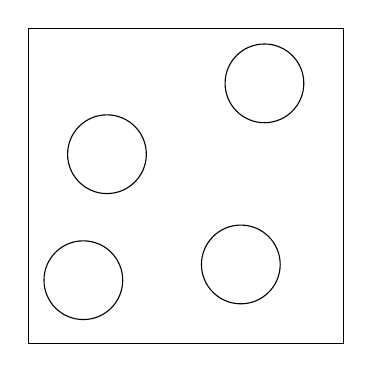
\begin{tikzpicture}
\draw (0,0) -- (4,0) -- (4,4) -- (0,4) -- (0,0);
\draw (.7,.8) circle (.5cm);
\draw (2.7,1) circle (.5cm);
\draw (1,2.4) circle (.5cm);
\draw (3,3.3) circle (.5cm);
\end{tikzpicture}
\end{center}

In all likelihood, you were immediately able to tell that the image contained four circles, and did not need to count them individually. However, try the same with the following image:\newline

\begin{center}
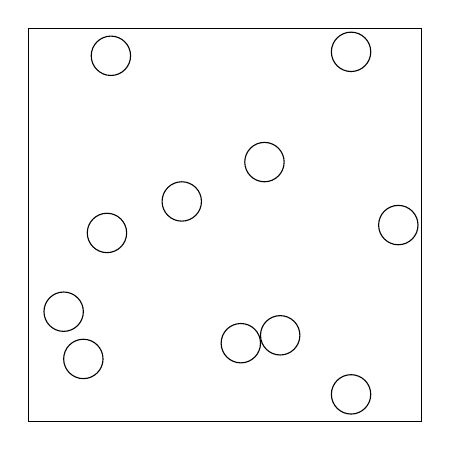
\begin{tikzpicture}
\draw (0,0) -- (5,0) -- (5,5) -- (0,5) -- (0,0);
\draw (.7,.8) circle (.25cm);
\draw (2.7,1) circle (.25cm);
\draw (1,2.4) circle (.25cm);
\draw (.45,1.4) circle (.25cm);
\draw (3.2,1.1) circle (.25cm);
\draw (3,3.3) circle (.25cm);
\draw (1.95,2.8) circle (.25cm);
\draw (4.1,.35) circle (.25cm);
\draw (1.05,4.65) circle (.25cm);
\draw (4.7,2.5) circle (.25cm);
\draw (4.1,4.7) circle (.25cm);
\end{tikzpicture}
\end{center}

This process likely required more effort than the first. Research into this cognitive process has shown that, in most people, ``the process of enumeration when there are more than 4 items, is slow (250-350 msec/item), effortful, and error-prone'' \cite{trick1994}. Even single-digit numbers of objects experience this increase in difficulty. Although the keys in RSA are not as easily visually representable as circles in a box, the numbers themselves can be greater than 600 digits, far above what a human can subitize. In the context of software, such as the program produced for this project, RSA can often be utilized without the user ever even seeing the keys. For hand-computation, however, those numbers would be the focus of numerous mathematical operations. A human being would not even be able to look at a large RSA key and easily know how many digits long it is, let alone be able to quickly comprehend its numerical value.

As a final thought on subitization, consider how it may interact with Miller's law. The astronomical size of common RSA keys would make them incredibly difficult, if not near impossible, to fully and accurately store in working memory or commit to longer-term memory. Breaking keys or other relevant values into chunks to make them easier to work with would almost certainly be required. However, if any portion of an equation is not written down before it is replaced in working memory it is at extremely high risk of being lost, leading to that equation portion needing to be performed again, with no inherently added security from the exact same issue arising the following time.
}
\end{itemize}

Upon seeing the size of the values used in RSA and the mathematical operations required, many would likely say it is sufficient to just call performing RSA by hand `difficult.' While this is undeniably true, the truth of the matter is much more scientific in nature and much more interesting. Human beings have genuine cognitive limitations that render such a task unfeasible, if not entirely impossible. There is a stark and important difference between claiming that something is too difficult, time consuming, or complicated, and claiming that the human mind has a factual and severe deficit in its ability to perform it. 


\section{Project Environment}
The environment of my project was fairly straightforward. Nearly all of the work was completed at my personal workstation in my home, with small exceptions of information gathering being performed on my laptop in the Pickler Memorial Library. The social environment was minimal, as all of the work was performed by myself. There were periodic meetings with Dr. Jaiswal to provide updates of project status and exchange information on potential additional features. The development environment largely utilized an agile process mindset. Changes and additions were made in small increments, and each issue was treated atomically. Focus would remain on each individual problem until they were resolved, rather than moving on and returning later.

\section{Other Involved Parties}
I worked with others to a rather minimal extent. Beyond my interactions with Dr. Jaiswal, the entirety of the project was planned and executed by me. In order to ensure the software was usable by individuals unfamiliar with RSA, I had several non-technologically-savvy people use the program and inform me of what they felt was straightforward and what features they felt needed further clarification.

\section{Hardware/Software Platform}
Although I did perform some information gathering and research on my laptop, the entirety of actual programming was performed on my desktop computer. In terms of hardware, it far exceeded any and all requirements for this project. It contains an Intel i7 4790k processor (4 cores, 8 threads, and a clock rate of 4.0 GHz), 8GB of DDR3 RAM, and an Asus Maximus VI motherboard. The operating system it runs on is Windows 7 Home Premium 64-bit, but in order to ensure fewer compatibility issues with UNIX-like systems, I did not use Visual Studio or other forms of native Windows C++. Instead, I utilized MinGW, a development environment that simulates GNU on Windows platforms and allowed me to compile my code with gcc. To actually write the code, I utilized the Atom text editor with a gcc compiler plugin. In order to keep track of the project as it developed, I made use of git, often through the interface provided by the application GitKraken.

\section{Communication Skills}
In order to communicate with my supervisor, Dr. Jaiswal, I relied primarily on email and in-person meetings. Minimal code was shared over our correspondence, but general topics and specific implementation issues were discussed in a general sense. The ability to discuss code in a concise and descriptive manner that I have developed over my time as a student proved to be extremely useful. When working with numbers as large as are utilized in RSA and the procedures to generate them, it quickly became clear how difficult speaking of the code relevant to them would be. Without the experience in working in groups and conveying implementation-specific information in a comprehensible manner that was imparted to me by my CS courses at Truman, this portion of the project would have led to considerable additional difficulties.

In order to find people to test my software, I largely relied on word of mouth and phone calls.

\section{Useful CS Courses \& Topics}
\begin{itemize}
\item{\textbf{CS 250 - Systems Programming.} The knowledge that CS 250 imparted to me about bitwise operations and lower-level programming proved invaluable in the creation of my SHA class.}
\item{\textbf{CS 260 - Object-Oriented Programming and Design.} Principles of object-oriented programming, especially that of encapsulation and atomic classes, facilitated efficient and effective interactions between the classes I designed.}
\item{\textbf{CS 370 - Software Engineering.} Without my knowledge and usage of Git, which I first became familiar with in this course, there were a number of times were I may have suffered data loss. Equally importantly, knowing how to manage such large and complex code as was necessary for this project would have proven immeasurably more difficult without the techniques taught in this course. Finally, the skills of talking about code and requirements in plain English to uninvolved parties I gained from CS 370 made correspondence with Dr. Jaiswal and my several testers much simpler.}
\item{\textbf{CS 390 - Operating Systems.} CS 390 showed me an area of computer science that I was largely unaware of prior to taking the course. Without understanding the specific differences between Windows and Linux, for example, making use of MinGW and the GMP library would have been a much more confusing process.}
\item{\textbf{CS 455 - Computer Security Fundamentals.} Without a doubt, CS 455 provided the foundation of this project for me. I was completely unaware of how interesting I would find the field of cybersecurity as a whole, and had no knowledge of the specifics of encryption systems such as RSA. Upon hearing of RSA in this course, I immediately knew that I would be interested in a capstone project involving it.}
\end{itemize}

\section{Useful Non-CS Courses \& Topics}
\begin{itemize}
\item{\textbf{MATH 263 - Analytic Geometry \& Calculus II, \& MATH 285 - Matrix Algebra.} Without the upper-level mathematical concepts taught in these courses, the idea of working with numbers larger than a quattuorducentillion would be absolutely unfathomable to me.}
\end{itemize}

\section{Lessons Learned}

\begin{enumerate}
\item
{
\textbf{Know what you're going to make before you make it.} Over the course of this program's development, a considerable number of changes were made to the intended end-product. Due to this, time spent researching was wasted, well-designed code was scrapped, and conflicting information gathered caused confusion. Although changes to the specific intentions and goals of a program are often inevitable, a more formalized plan of my end goals being prepared from the beginning would have saved a lot of expended time and effort.
}
\item 
{
\textbf{Test portions of large programs in small parts.} This was a principle I learned in CS 370, but as this project has easily been the largest programming project I have ever completed, this lesson was quite strongly reinforced for me. The nested nature of many of my functions, in addition to the complexity of the mathematics being performed and the sometimes unclear FIPS specifications, made unit testing and other function-specific testing difficult. Although I did perform testing to a considerable extent, additional time spent planning more complete tests would have, despite taking more time initially, saved me time in the long run.
}
\item
{
\textbf{Coding in accordance with external specifications can be difficult, to say the least.} Writing my program in alignment with FIPS specifications was an arduous process. Sometimes, the meaning of a particular statement or mathematical expression was incredibly unclear. The symbols of variables and operators were sometimes inconsistent, occasionally within the same publication and very often between publications. Although I am quite sure that -- and as I experienced in CS 370 -- programming according to commercial, client requirements is quite different from doing so according to federal standards, the lesson is the same: Producing something according to needs sourced from a third party can lead to countless opportunities for confusion, misinterpretation, and improper results.
} 
\end{enumerate}

\section{Problems \& Solutions}
\begin{itemize}
\item
{
\textbf{Windows Compatibility.} Upon beginning this project, it became immediately apparent that I was going to need to make use of an external C++ library to allow for arithmetic on numbers with a bitlength of 2048 or larger. After exploring several Windows-compatible options, the most notable being Matt McCutchen's Big Integer Library, and encountering only broken/poorly-documented code and compatibility issues, I concluded that I would need to explore other options. I elected to use GMP, which enjoys a very strong reputation as a multiprecision arithmetic library. However, due to its GNU affiliationn GMP only runs cleanly with gcc. In order to utilize gcc on a Windows machine, I installed MinGW, a software development environment that allows for the use of gcc. Despite an unclear and complicated install process and a few additional compatibility issues that had to be addressed, GMP was clearly the best choice for my purposes. Knowing this, I maintained efforts until I had a fully-functional install of the library and was able to proceed with the project.
}
\item
{
\textbf{Nested Requirements.} As I read deeper into the FIPS publications and their specifications, I repeatedly found additional requirements within requirements. One publication would instruct me to seek information located in another publication, and the second publication would then point me elsewhere. Collecting all of the documentation I required -- especially when a comprehensive list of what I would need was completely unavailable, and was scattered across numerous publications -- was like following a bread trail. The only option was to deeply and completely scan the relevant areas of each text as I found them, until any directions to other publications pointed to information that I already had obtained. Given that some of these publications are hundreds of pages long, this was no easy task, but I continued until I was certain I had gathered all of the information I would need to meet FIPS guidelines. 
}
\item
{
\textbf{Lack of FIPS-Compliant Resources.} Under FIPS standards, there are numerous cases where, if code that is intended to be FIPS-compliant relies on code that is not FIPS-compliant, the compliance for the entire program is nullified. This was the case for the use of SHA and random number generators for RSA. My initial intention was not to create my own classes for these purposes. However, searching online for external code or libraries I could make use of, I could not find any that provided the functionality I needed, was definitively FIPS-compliant, did not cost a small fortune, and would not add a host of legal implications as a result of its use. Being as close to FIPS-compliant as was feasible was one of the core intentions of my project from its early stages, so rather than accept a large-scale decrease in compliance, I elected to dig up yet more FIPS documentation and create my own classes to suit my needs.
}
\end{itemize}


\section{Things I Wish I had Known}
\begin{itemize}
\item
{
\textbf{GMP, a library designed for C, does in fact have an extended C++ library.} In my initial attempts to create this program, I was of the belief that, although incredibly powerful, the GMP library only provided structs that had access to the multiprecision functions. This caused sections of code that would ordinarily take only one line require several more -- generally around four, but occasionally much higher. The way that access to stored variables and functions was structured -- a very traditionally C-programming manner -- made the code much less easily readable, leading to my own code occasionally being difficult for even me to understand, despite my best efforts to comment and document dutifully.

After struggling greatly with debugging this code, I decided to look more deeply into the GMP documentation, and discovered an extended library that incorporates all of the multiprecision functionality into C++ classes. This easily halved the number of lines in my code, and even more importantly made mathematical expressions appear much more natural and readable. Although changing my code to make use of the C++ classes resulted in a much cleaner and higher-quality product, it required removal of large portions of code that had taken a great deal of time to produce, and even further time adding the new code in. That said, working with the complex equations making use of the original, much less descriptive  GMP code resulted in me analyzing the mathematical functions to a much greater degree and obtaining a much deeper understanding of what was actually being performed. In the end, knowledge of this beforehand would have saved a great deal of time, but I likely would not have such a strong comprehension of what my program is actually performing.
}

\item
{
\textbf{Creation of GUIs is incredibly complex.} For some time, I had planned for this program to implement an aesthetically pleasing and easy to use GUI. At separate times, I had attempted to use both WxWidgets and Qt to create a GUI, and both times quickly found myself in over my head. I persisted, however, and all I ended up achieving was confusing myself and modifying my code in detrimental ways -- thanks to Git, no permanent damage was done. GUI programming is an art and a craft in itself, and had I known the immense difficulty associated with it beforehand, I would have been aware that creating a GUI, at least in C++, would be a project in itself and likely draw attention away from the true intention of my program.
}
\end{itemize}

\section{Results: Anticipated vs. Actual}
After all has been said and done, I am very pleased with the end result of this project. The cryptosystem tool works perfectly in terms of its intended operations, and exhibits no errors that I or my testers have been able to find (while I am aware that testing can only show the presence of bugs, rather than a lack of them). My initial hopes for the project, looking back, were quite grandiose, and I now know that they could easily be described as overly ambitious. 

Initially, I had envisioned a cryptosystem tool with a fully functioning GUI that could demonstrate encryption/decryption or signing/authentication between two separate ciphers, including showing what would occur if incorrect keys were utilized. I also had ideas of being able to demonstrate this via two instances of the program connected over a network. However, as soon as the difficulty of creating a GUI became apparent, devising an approach to this that would be easily-interpretable while still being constrained to the command line seemed unlikely. Additionally, I severely underestimated how complicated the procedures outlined in the FIPS publications would be. I had pictured it as being a number of additions to the simple series of equations presented to me in CS 455, while the reality of it was a volume of additional steps that were much more difficult for me to understand than the core equations. All of this led to me canceling those plans, and placing emphasis on a command-line based, security-focused cryptosystem.

While I one day would very much enjoy being able to return to this project and add some of the functionality that I ended up having to scrap, as of right now I strongly feel that the product of this capstone is an appropriate culmination of my time as a computer science student at Truman. It required hours of research and coding, success and failure, pride and frustration, and most of all testing and improving. I certainly have never faced such a difficult programming before, and believe that, given my final product, I have tackled it to an extent that has made me very proud to call this work my capstone.

\singlespacing
\bibliographystyle{apalike}
\bibliography{wood_bibliography}

\end{document}